\documentclass[UTF8,11pt]{ctexart}
\usepackage[a4paper,margin=22mm]{geometry}
\usepackage{graphicx,enumitem,amssymb,tabularx}
\usepackage[normalem]{ulem}
\usepackage{xeCJKfntef}
\setlength{\parindent}{0pt}
\setlength{\parskip}{.6em}
\sloppy
\begin{document}
\section*{2021年6月英语四级真题(第3套)}
\subsection*{2021年6月大学英语四级考试真题（三）}


\subsection*{Part I Writing (30 minutes)}


Directions: For this JJ(lrt , you are allowed 80 minutes to write an es皿ytitled "Do吻lent志eogames l已to 吻lence? ". The statement given below is for your reference . You should write at least丝Q\_ words but no more than型words. A growing body of res纽rch finds t血t吻lent诅eo games can mtike应s act aggressively in their real world relationships, causing an increase in吻lence.


\subsection*{Part I Listening Comprehension (25 minutes)}


说明：由千2021年6月四级考试全国共考了两套听力，本套真题听力与前两套内容相同，只是选项顺序不同，因此在本套真题中不再重复出现。


Part ][ Reading Comprehension (40 minutes)


\subsection*{Section A}


Directions: In this 亚ction, there is a pas. 皿ge with ten blanks. You are required to select one word for each


\subsection*{blank from a l比t of choices given in a wotd bank following the pas. 皿ge. Read the pas. 皿ge through carefully}


before making your choices. 压h choice in the bank is identified by a letter. Please mark the com芍劝uling


\noindent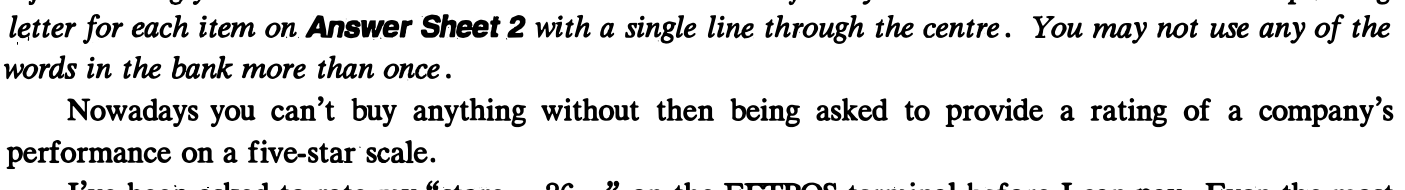
\includegraphics[width=\linewidth,height=.8\textheight,keepaspectratio]{2021-06-03.assets/char-001-line-010.png}\par

I've been asked to rate my "store 26 " on the EFfPOS terminal before I can pay. Even the most 27 activities, such as calling Telstra or \textbf{picking }up a parcel from Australia Post, are followed by texts or emails with surveys asking, 飞ow did we do?"


0血e purchases are 28 followed up by a customer satisfaction survey. Companies are so 29 for a hit of stars that if you delete the survey the company sends you another one.


We're 30 to rate our apps when we've barely had a chance to use them. One online course provider I use asks you what you think of the course after you've only completed \_包\_31 2 per cent of it.


Econom尪t Jason Murphy says that companies use customer satisfaction ratings because a 32 display of star feedback has become the nuclear power sources of the modem economy.


\noindent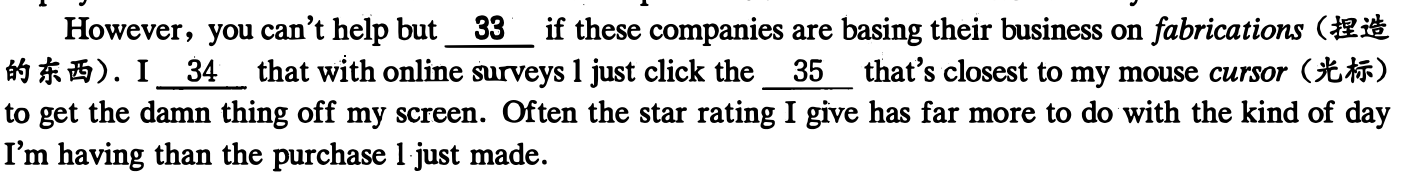
\includegraphics[width=\linewidth,height=.8\textheight,keepaspectratio]{2021-06-03.assets/char-001-line-015.png}\par

\begin{itemize}[leftmargin=2em,itemsep=.2em,topsep=.4em]\item[A.] announce
\item[B.] commonplace
\item[C.] confess
\item[D.] desperate
\item[E.] experience
\item[F.] fascinated
\item[G.] option
\item[H.] prompted
\item[I.] roughly
\item[J.] routinely 0) wonder
\item[K.] shining
\item[L.] showering
\item[M.] variety
\item[N.] voyage
\end{itemize}

\subsection*{\textbf{Section }B}


\textbf{Directions: In this section, you are going to read a passa.ge with ten statements attached to it. F.ach} \textbf{statement contains information given in one of the paragraphs. Identify the paragraph from which the} \textbf{对ormation is derived. You may choose a paragraph more than once. F.ach paragraph is marked with a} \textbf{letter. Answer the questions by marking the correspa叫ing letter on Answer Sheet 2.} \textbf{Science of} 瞬\textbf{tba心：How failure can屿10\textbackslash{}le career prospects}


A) \textbf{How do early career setbacks affect our long-term success? Failures can help us learn and overcome our} \textbf{fears. But disasters can still wound us. They can screw us up and set us back. Wouldn't it be nice if} \textbf{there was genuine, scientifically documented truth to the expression "what doesn't kill you makes you} \textbf{stronger''?}


B) \textbf{One way social scientists have probed the effects of career setbacks is to look at scientists of very} \textbf{similar qualifications. These scientists, for reasons that are mostly arbitrary, either just missed getting} \textbf{a research grant or just barely made it. In social sciences, this is known as examining "near misses" and} \textbf{"narrow wins" in areas where merit is subjective. That allows researchers to mea亚e only the effects} \textbf{of being chosen or not. Studies in this area have found conflicting results. In the competitive game of} \textbf{biomedical science, research has been done on scientists who narrowly lost or won grant money. It} \textbf{suggests that narrow winners become even bigger winners down the line. In other words, the rich get} \textbf{richer.}


C) \textbf{A 2018 study published in the Proceedi鸣'S of the National Academy of Sciences, for example, followed} \textbf{researchers in the Netherlands. Researchers concluded that those who just barely qualified for a grant} \textbf{were able to get twice as much money within the next eight years as those who just missed out. And the} \textbf{narrow winners were 50 percent more likely to be given a professorship.}


D) \textbf{Others in the US have found similar effects with National Institutes of Health early-career fellowships} \textbf{launching narrow winners far ahead of close losers. The phenomenon is often referred to as the} \textbf{Matthew effect, inspired by the Bible's wisdom that to those who have, more will be given. There's a} \textbf{good explanation for the phenomenon in the book匹Formula: The Universa.l La}泗\textbf{of Success by} \textbf{Albert Laszlo Barabasi. According to Barabasi, it's easier and less risky for those in positions of power}


\noindent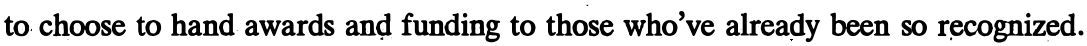
\includegraphics[width=\linewidth,height=.8\textheight,keepaspectratio]{2021-06-03.assets/char-002-line-006.png}\par

E) \textbf{This is bad news for the losers. Small early career setbacks s氏m to have a disproportionate effect} \textbf{down the line. What didn't kill them made them weaker. But other studies using the same technique} \textbf{have shown there's sometimes no penalty to a near miss. Students who just miss getting into top high} \textbf{schools or universities do just as well later in life as those who just manage to get accepted. In this case,} \textbf{what didn't kill them simply didn't matter. So is there any evidence that setbacks might actually} \textbf{improve our career prospects? There is now.}


F) \textbf{In a study published in Nature Communications, Northwestern University sociologist Dashun Wang} \textbf{tracked more than 1, 100 scientists who were on the border between getting a grant and missing out} \textbf{between 1990 and 2005. He followed various measures of performance over the next decade. These} \textbf{included how many papers they authored and how influential those papers were, as measured by the} \textbf{number of subsequent citations. As expected, there was a much higher rate of attrit加（减员）among}


\textbf{scientists who didn't get grants. But among those who stayed on, the close losers performed even better} \textbf{than the narrow winners. To malce sure this wasn't by chance,'Wang conducted additional tests using} \textbf{different performance measures. He examined how many times people were first authors on influential} \textbf{studies, and the like.}


G) \textbf{One straightforward reason close losers might outperform narrow winners is that the two groups have} \textbf{comparable ability. In Wang's study, he selected the most determined, passionate scientists from the} \textbf{loser group and culled (剔除）what he deemed the wealcest members of the winner group. Yet the} \textbf{persevering losers still came out on top. He thinks that being a close loser m烛t give people a} \textbf{psychological boost, or the proverbial kick in the pants.}


H) \textbf{Utrecht University sociologist Arnout van de Rijt was the lead author on\_ the 2018 paper showing the} \textbf{rich get richer. He said the new finding is apparently reasonable and worth some attention. His own} \textbf{work showed that although the narrow winners did get much more money in the near future, the actual} \textbf{performance of the close losers was just as good.}


I) \textbf{He said the people who should be paying regard to the Wang paper are the funding agents who} \textbf{distribute government grant money. After all, by continuing to pile riches on the narrow winners, the} \textbf{taxpayers are not getting the maximum bang for their buck if the close losers are performing just as} \textbf{well or even better. There's a huge amount of time and effort that goes into the process of selecting}


\noindent
\includegraphics[width=\linewidth,height=.8\textheight,keepaspectratio]{2021-06-03.assets/char-003-line-004.png}\par

\textbf{good at distributing money. "Maybe we should spend less money trying to figure out who is better than} \textbf{who," he函d, suggesting that some more equal dividing up of money might be more productive and}


\noindent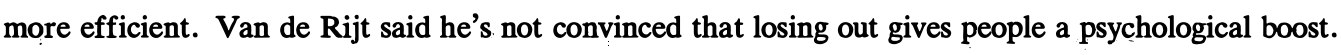
\includegraphics[width=\linewidth,height=.8\textheight,keepaspectratio]{2021-06-03.assets/char-003-line-006.png}\par

\textbf{It may yet be a selection effect. Even though Wang tried to account for this by culling the we吐est} \textbf{winners, it's impossible to know which of the winners would have quit had they found themselves on} \textbf{the losing side.}


\noindent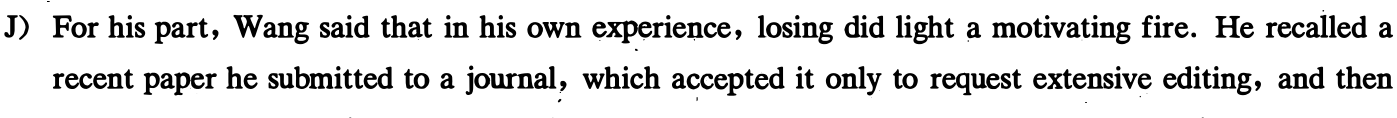
\includegraphics[width=\linewidth,height=.8\textheight,keepaspectratio]{2021-06-03.assets/char-003-line-008.png}\par

\textbf{reversed course and rejected it. He submitted the unedited version to a more respected journal and got} \textbf{accepted.}


\noindent
\includegraphics[width=\linewidth,height=.8\textheight,keepaspectratio]{2021-06-03.assets/char-003-line-010.png}\par

\textbf{better. We regard these disappointments as a (ate we could have avoided with more careful}


\noindent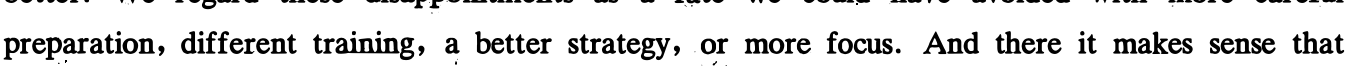
\includegraphics[width=\linewidth,height=.8\textheight,keepaspectratio]{2021-06-03.assets/char-003-line-012.png}\par

\textbf{failures show us the road to success. These papers deal with a kind of failure people have little control} \textbf{over--rejection. Others determine who wins and who loses. B11t at the very least, the research is} \textbf{starting to show that early setbacks don't have to be fatal. They might even m吐e us better at our jobs.} \textbf{Getting paid like a w.inner, though? TI沮's a .different matter.}


\textbf{36. Being a close loser could greatly motivate one to persevere in their research.}


\textbf{37. Grant awarders tend to favor researchers already recognized in their respective fields.}


\textbf{38. Suffering early setbacks might help people improve their job performance.}


\textbf{39. Research by social scientists on the effects of career setbacks has produced contradictory findings.}


\textbf{40. It is not to the best interest of taxpayers to keep giving money to narrow winners.}


\textbf{41. Scientists who persisted in research without receiving a grant made greater achievements than those}


\textbf{who got one with luck, as suggested in one study.}


\textbf{42. A research paper rejected by one journal may get accepted by another.}


\textbf{43. According to one recent study, narrow winners of research grants had better chances to be promoted}


\textbf{to professors.}


\textbf{44. One researcher suggests it might be more fruitful to distribute grants on a relatively equal basis.}


\textbf{45. Minor setbacks in their early career may have a strong negative effect on the career of close losers.}


\subsection*{\textbf{Section C}}


\textbf{Directions: There are 2 passages in this section. 应ch passage is followed by some questions or unfinished} \textbf{statements. For each of them there are four choices marked A), B), C) and D). You should decide on the} \textbf{best choice and mark the co}汀\textbf{esponding letter on Answer Sheet 2 with a single line through the centre.}


\subsection*{\textbf{Passage One}}


\textbf{Questions 46 to 50 are based on the following passage.}


\noindent
\includegraphics[width=\linewidth,height=.8\textheight,keepaspectratio]{2021-06-03.assets/char-004-line-012.png}\par

\textbf{well as mental health. It is found that people are more creative following\textperiodcentered{}the completion of a tedious task.} \textbf{When people are bored, they have an increase in "associative thought"一the process of making new} \textbf{connections between ideas, which is linked to innovative thinking. These studies are impressive, but in} \textbf{reality, the benefits of boredom may be related to having time to clear your mind, be quiet, or daydream.}


\textbf{In our stimulation-rich world, it seems unrealistic that boredom could occur at all. Yet, there are} \textbf{valid reasons boredom may feel so p血ul. As it turns out, boredom might signal the fact that you have a} \textbf{need that isn't being met.}


\textbf{Our always-on world of social media may result in more connections, but they are superficial and can} \textbf{get in the way of building a real sense of belonging. Feeling bored may signal the desire for a greater sense} \textbf{of community and the feeling that you fit in with others around you. So take the step of joining an} \textbf{organization to build face-to-face relationships. You'll find depth that you won't get from your screen no} \textbf{matter how many likes you get on your post.}


\textbf{Similar to the need for belonging, bored people often report that they feel a limited sense of} \textbf{meaning. It's a fundamental human need to have a larger purpose and to feel like we're part of something} \textbf{bigger than ourselves. When people are bored, they're more likely to feel less meaning in their lives. If} \textbf{you want to reduce boredom and increase your sense of meaning, seek work where you can make a unique} \textbf{contribution, or find a cause you can support with your time and talent.}


\textbf{If your definition of boredom is being quiet, mindful, and reflective, keep it up. But if you're} \textbf{struggling with real boredom and the emptiness it provokes, consider whether you might seek new} \textbf{connections and more significant challenges. These are the things that will genuinely relieve boredom and} \textbf{make you more effective in the process.}


\textbf{46. What have studies found about boredom?}


\begin{itemize}[leftmargin=2em,itemsep=.2em,topsep=.4em]\item[A.] \textbf{It facilitates innovative thinking.}
\item[B.] \textbf{It is a result of doing boring tasks.}
\end{itemize}

\begin{itemize}[leftmargin=2em,itemsep=.2em,topsep=.4em]\item[C.] \textbf{It helps people connect with others.}
\item[D.] \textbf{It does harm to one's mental health.}
\end{itemize}

\textbf{47. What does the author say boredom might indicate?}


\begin{itemize}[leftmargin=2em,itemsep=.2em,topsep=.4em]\item[A.] \textbf{A need to be left alone.}
\item[B.] \textbf{A desire to be fulfilled.}
\item[C.] \textbf{A conflict to be resolved.}
\item[D.] \textbf{A feeling to be validated.}
\end{itemize}

\textbf{48. What do we learn about social media from the passage?}


\begin{itemize}[leftmargin=2em,itemsep=.2em,topsep=.4em]\item[A.] \textbf{It may be an obstacle to expanding one's connections.}
\item[B.] \textbf{It may get in the way of enhancing one's social status.}
\item[C.] \textbf{It may prevent people from developing a genuine sense of community.}
\item[D.] \textbf{It may make people feel that they ought to fit in with the outside world.}
\end{itemize}

\textbf{49. What does the author suggest people do to get rid of boredom?}


\begin{itemize}[leftmargin=2em,itemsep=.2em,topsep=.4em]\item[A.] \textbf{Count the likes they get on their posts.}
\item[B.] \textbf{Reflect on how they relate to others.}
\item[C.] \textbf{Engage in real-life interactions.}
\item[D.] \textbf{Participate in online discussions.}
\end{itemize}

\textbf{50. What should people do to enhance their sense of meaning?}


\begin{itemize}[leftmargin=2em,itemsep=.2em,topsep=.4em]\item[A.] \textbf{Try to do something original.}
\item[B.] \textbf{Confront significant challenges.}
\item[C.] \textbf{Define boredom in their unique way.}
\item[D.] \textbf{Devote themselves to a worthy cause.}
\end{itemize}

\subsection*{\textbf{Passage Two}}


\textbf{Questions 51 to 55 are based on the following passage.}


\textbf{Can you remember what you ate yesterday? If asked, most people will be able to give a vague} \textbf{description of their main meals: breakfast, lunch, dinner. But can you be sure you've noted every snack} \textbf{bar in your car, or every handful of nuts at your desk? Most people will have a feeling that they've missed} \textbf{something out.}


\textbf{We originally had this suspicion back in 2016, puzzled by the fact that national statistics showed} \textbf{calorie consumption falling dramatically over past decades. We found reliable evidence that people were} \textbf{drastically under-reporting what they ate.}


\textbf{Now the Office for National Statistics has confirmed that we are consuming 50\% more calories than} \textbf{our national statistics claim.}


\textbf{Why is this happening? We can point to at least three potential causes. One is the rise\_ in obesity levels} \textbf{itself. Under-reporting rates are much higher for obese people, because they simply consume more food,} \textbf{and thus have more to remember.}


\textbf{Another cause is that the proportion of people who are trying to lose weight has been increasing over} \textbf{time. People who want to lose weight are more 1ilcely to under-report their eating—regardless of whether} \textbf{they are overweight or not. This may be driven partly by self-deception or "wishful thinkin旷}


\textbf{The final potential cause is an increase in snacking and eating out over recent decades—both in terms} \textbf{of how often they happen and how much they contribute to our overall energy intake. Again, there is} \textbf{evidence that food consumed out of the home is one of the most poorly recorded categories in surveys.}


\textbf{So, what's the message conveye .d? For statistics, we should invest m more accurate measurement} \textbf{options. For policy, we need to focus on options that make it easy for people to eat fewer calories. If} \textbf{people do not know how much they are eating, it can be really hard for them to stick to a diet. Also, we} \textbf{should be looking for new ways to ensure what people eat wouldn't have much impact on their waistlines.} \textbf{If this works, it won't matter if they can't remember what they ate yesterday.}


\textbf{51. What did the author suspect back in 2016?}


\begin{itemize}[leftmargin=2em,itemsep=.2em,topsep=.4em]\item[A.] \textbf{Calorie consumption had fallen drastically over the decades.}
\item[B.] \textbf{Most people surveyed were reluctant to reveal what they ate.}
\item[C.] \textbf{The national statistics did not reflect the actual calorie consumption.}
\item[D.] \textbf{Most people did not include snacks when reporting their calorie intake.}
\end{itemize}

\textbf{52. What has the Office for National Statistics verified?}


\begin{itemize}[leftmargin=2em,itemsep=.2em,topsep=.4em]\item[A.] \textbf{People's calorie intake was far from accurately reported.}
\item[B.] \textbf{The missing out of main meals leads to the habit of snacking.}
\item[C.] \textbf{The nation's obesity level has much to do with calorie intake.}
\item[D.] \textbf{Calorie consumption is linked to the amount of snacks one eats.}
\end{itemize}

\textbf{53. What do we learn about obese people from the passage?}


\begin{itemize}[leftmargin=2em,itemsep=.2em,topsep=.4em]\item[A.] \textbf{They usually keep their eating habits a secret.}
\item[B.] \textbf{They overlook the potential causes of obesity.}
\item[C.] \textbf{They cannot help eating more than they should.}
\item[D.] \textbf{They have difficulty recalling what they have eaten.}
\end{itemize}

\textbf{54. What often goes unnoticed in surveys on food consumption?}


\begin{itemize}[leftmargin=2em,itemsep=.2em,topsep=.4em]\item[A.] \textbf{The growing trend of eating out.}
\item[B.] \textbf{The potential causes of snacking.}
\item[C.] \textbf{People's home energy consumption.}
\item[D.] \textbf{People's changing diet over the years.}
\end{itemize}

\textbf{55. What does the author suggest policymakers do about obesity?}


\begin{itemize}[leftmargin=2em,itemsep=.2em,topsep=.4em]\item[A.] \textbf{Remind people to cut down on snacking.}
\item[B.] \textbf{Make sure people eat non-fattening food.}
\item[C.] \textbf{Ensure people don't miss their main meals.}
\item[D.] \textbf{See that people don't stick to the same diet.}
\end{itemize}

\subsection*{Part N Translation (30 minutes)}


\textbf{Directions: For this part, you are allowed 30 minutes to translate a passage from Chinese into English. You} \textbf{should write your answer on Answer Sheet 2.}


\textbf{垄(Longjing)是一种绿茶，主要产自中国东部沿海的浙江省。} \textbf{龙井茶独特的香味和口感为其赢得了} \textbf{”的称号，在中国深受大众的欢迎，在海外饮用的人也越来越多。 龙井茶通常手工制作，其价格} \textbf{“中国名茶可能极其昂贵，也可能比较便宜，这取决于茶的生长地、采摘时间和制作工艺。 龙井茶富含维生素C和其他多种有益健康的元素。 经常喝龙井茶有助于减轻疲劳、延缓衰老。}

\end{document}